%%%%%%%%%%%%%%%%%%%%%%%%%%%%%%%%%%%%%%%%%%%%%%%%%%%%%%%%%%%%%%%%%%%%%%%%
%    INSTITUTE OF PHYSICS PUBLISHING                                   %
%                                                                      %
%   `Preparing an article for publication in an Institute of Physics   %
%    Publishing journal using LaTeX'                                   %
%                                                                      %
%    LaTeX source code `ioplau2e.tex' used to generate `author         %
%    guidelines', the documentation explaining and demonstrating use   %
%    of the Institute of Physics Publishing LaTeX preprint files       %
%    `iopart.cls, iopart12.clo and iopart10.clo'.                      %
%                                                                      %
%    `ioplau2e.tex' itself uses LaTeX with `iopart.cls'                %
%                                                                      %
%%%%%%%%%%%%%%%%%%%%%%%%%%%%%%%%%%
%
%
% First we have a character check
%
% ! exclamation mark    " double quote
% # hash                ` opening quote (grave)
% & ampersand           ' closing quote (acute)
% $ dollar              % percent
% ( open parenthesis    ) close paren.
% - hyphen              = equals sign
% | vertical bar        ~ tilde
% @ at sign             _ underscore
% { open curly brace    } close curly
% [ open square         ] close square bracket
% + plus sign           ; semi-colon
% * asterisk            : colon
% < open angle bracket  > close angle
% , comma               . full stop
% ? question mark       / forward slash
% \ backslash           ^ circumflex
%
% ABCDEFGHIJKLMNOPQRSTUVWXYZ
% abcdefghijklmnopqrstuvwxyz
% 1234567890
%
%%%%%%%%%%%%%%%%%%%%%%%%%%%%%%%%%%%%%%%%%%%%%%%%%%%%%%%%%%%%%%%%%%%
%
\documentclass[10pt]{iopart}
%\documentclass[12pt]{iopart}
%\newcommand{\gguide}{{\it Preparing graphics for IOP Publishing journals}}
%Uncomment next line if AMS fonts required
%\usepackage{iopams}
\usepackage{graphicx}
\usepackage{multirow}
\usepackage{amssymb}
\usepackage{url}
\begin{document}

\title[Computer vision for quantifying Fe-related defects in Si solar cell]{Computer vision-based method for quantifying iron-related defects in silicon solar cell}

\author{Oleg Olikh\footnote{Author to whom any correspondence should be addressed.}, Oleksii Zavhorodnii, Yulia Perets}

\address{Taras Shevchenko National University of Kyiv, Kyiv 01601, Ukraine}

\ead{olegolikh@knu.ua}
%\vspace{10pt}
%\begin{indented}
%\item[]August 2017
%\end{indented}

\begin{abstract}
abstract abstract abstract abstract abstract abstract
\end{abstract}

%
% Uncomment for keywords
\vspace{2pc}
\noindent{\it Keywords}: defect, Si solar cell, iron contamination, machine learning, computer vision

% Uncomment for Submitted to journal title message
\submitto{\SST}
%
% Uncomment if a separate title page is required
%\maketitle

% For two-column output uncomment the next line and choose [10pt] rather than [12pt] in the \documentclass declaration
\ioptwocol
%


\section{Introduction}\label{sec:Int}

Due to the urgent need to address environmental challenges and the growing global demand for renewable energy, the deployment of photovoltaic (PV) systems has been rapidly increasing worldwide.
In particular, solar PV generation exceeded 1,600 TWh in 2023 \cite{IEA2024Renewables, OSAMA2025}, rose by about 30\% in 2024 \cite{Prometheus2025}, and forecasts indicate that total installed capacity will surpass 6 TW by 2030 \cite{IEA2024Renewables}.
Meanwhile, crystalline silicon photovoltaics, which have benefited from decades of scientific advancement and continuous cost reductions, continued to dominate the market in 2024, accounting for approximately 98\% of the global share \cite{Fischer2025ITRPV, THOME2025}.

As in other semiconductor devices, defects play a decisive role in determining the operating parameters of solar cells.
Therefore, diagnosing defects, particularly determining their concentrations, is critically important for maintaining the stable performance of PV systems.
In recent years, researchers have increasingly complemented established defect-characterisation methods with machine learning (ML) approaches that improve the accuracy, speed, and cost efficiency of these analyses.
The use of ML methods for analysing macroscopic defects (such as cracks, finger failures, hotspots, and scratches) and point defects, however, differs significantly.
Researchers typically detect macroscopic defects in PV systems using two main approaches \cite{Jia2024, Hijjawi2023}.
The first approach, Electrical Testing Techniques, involves analysing characteristic electrical curves of parameters such as current, voltage, and power.
The second approach, Imaging-Based Techniques, involves analysing electroluminescence (EL) \cite{Liu2024a} or photoluminescence \cite{Doll2021} images of solar cells.
Numerous review studies demonstrate extensive use of ML in both approaches \cite{Datta2023, Jaiswal2023, Buratti2024, MAHDAVIPOUR, Hopwood2020, Li2021, Liu2021}.

Regarding point defects, although they represent one of the primary limitations of PV devices, researchers have developed considerably fewer ML techniques specifically for their analysis.
Existing ML-based approaches include extracting recombination-active centre parameters from lifetime measurements \cite{Wang2024a, Buratti2022, Buratti2020a},
detecting radiation-induced defects using Raman spectroscopy \cite{Park2022, Chia2024},
estimating the concentration of contaminant impurities from the ideality factor of current–voltage characteristics \cite{Olikh2022PPV},
and analysing variations in photovoltaic conversion parameters \cite{Olikh2025SE}.
Nevertheless, a relatively limited number of such methods are offered.


One of the main challenges in applying ML methods effectively is that training the models requires a large amount of labelled data \cite{Buratti2024}.
In practice, researchers often cannot obtain such large volumes of experimental data;
therefore, they commonly employ approaches such as simulations,
in which hundreds of thousands of dependencies are computed \cite{Wang2024a, Buratti2022, Buratti2020a, Olikh2025MSEB, Olikh2025SE};
Physics-Informed Neural Networks (PINNs), which incorporate physical laws into the loss function to generate synthetic data \cite{Wang2024b, Li2025};
or Transfer Learning, in which a model trained on one task is adapted to another related task \cite{Kaya2019, Kim2023}.
However, simulations can be highly demanding in terms of time and computational resources; PINNs are primarily suitable for phenomena described by partial differential equations, and pre-trained models are not available for all types of physical problems.
At the same time, one of the most extensively studied tasks in machine learning is computer vision (CV),
for which many pre-trained models have been publicly released.
Moreover, these models are typically trained on extremely large standard datasets.
For example, EfficientNetB7 was trained on approximately 1.2 million images from the ImageNet dataset.

This work primarily aimed to apply standard pre-trained CV models to analyse electrophysical measurement results related to point defects.
In particular, we focused on quantifying iron in boron-doped crystalline silicon solar cells by examining the short-circuit current
($I_\mathtt{SC}$) relaxation following intense illumination.
Iron represents one of the most prevalent, ubiquitous, and efficiency-limiting metallic impurities in such structures \cite{Buonassisi2006, IronSC},
which, as noted earlier, form the foundation of the photovoltaic market.
In Si:B, iron tends to form iron–boron pairs under equilibrium conditions, which intense illumination can dissociate \cite{Kimerling1983, FeBAssJAP2014}.
In fact, the aforementioned $I_\mathtt{SC}$ variations directly reflect the recovery process of iron–boron pairs \cite{Olikh2021JAP}.


It should be noted that the use of well-established computer vision benchmark architectures such
as YOLO, MobileNetV2, EfficientNet, ResNet, Xception, GoogleNet, and other convolutional neural networks (CNNs) is a common approach for identifying macrodefects from EL
measurements \cite{Liu2024a, Li2024a, Jia2024, Otamendi2021, Chen2022, AlOtum2024, Abdelsattar2025, tella2025}.
However, in this case, the measurement result is an image, which makes the approach relatively straightforward.
In our case, it was necessary to transform the time dependence into an image representation.
Standard approaches to solving such problems involve the use of Fourier or wavelet transforms, and last were applied in this study.
In photovoltaics, wavelet transforms are typically used for processing solar cell images to enhance the detection of
macrodefects \cite{Li2012, Rosa2024}, but they can also be employed to convert one-dimensional non-stationary signals into two-dimensional spectrograms and thereby enable the effective extraction of subtle features \cite{Vinit2020}.

By applying computer vision models to wavelet spectrograms represented as images, we generated high-dimensional feature vectors and used them as inputs for traditional regression models.
The $I_\mathtt{SC}$(t) dependencies for training the regression models were obtained through both simulation and experimental measurements.
In both cases, the hybrid Transfer Learning approach produced predictions with sufficiently high accuracy (within a few percent), even when training models on small datasets containing fewer than 30 samples.
Importantly, the proposed approach is highly versatile and can be extended to a wide range of tasks related to defect characterization and other applications.


\section{Methodology}\label{sec:Exp}

\subsection{General outline of the method}\label{subsec:GenSch}

\Fref{Fig1} illustrates the workflow of the ML pipeline used to extract iron contamination from $I_\mathtt{SC}(t)$ dependencies.
The process consists of three main blocks: Data Acquisition, CNN Feature Processing, and Predictive Regression.
The first stage involves either simulating or experimentally measuring the time dependence
of the short-circuit current in a solar cell after the induced decay of FeB pairs.
These procedures are described in more detail in Subsections~\ref{subsec:SimDet} and \ref{subsec:ExpDet}.
For the experimental curves, the data were smoothed using a Savitzky–Golay filter \cite{Krishnan2013}.
Subsequently, a continuous wavelet transform \cite{Torrence1998} was applied to convert the one-dimensional time dependencies
into two-dimensional spectrograms represented as images,
where each point corresponds to the amplitude of the wavelet coefficient at a specific time and frequency.
The Morlet wavelet was employed, and the procedure was implemented using the Python package PyWavelets.
Examples of the resulting images are shown in \Fref{Fig2}b and \Fref{Fig2}c.
Data augmentation was then performed by flipping the images along the x- and y-axes and rotating them by 90$^{\circ}$, 180$^{\circ}$, and 270$^{\circ}$.
This procedure is known to improve the accuracy of ML model predictions, particularly when only small datasets are available \cite{Ahmad2020}.


\begin{figure*}

\includegraphics[width=0.95\textwidth]{Fig1}
\caption{\label{Fig1}
The workflow of the ML pipeline
}%
\end{figure*}

\begin{figure}
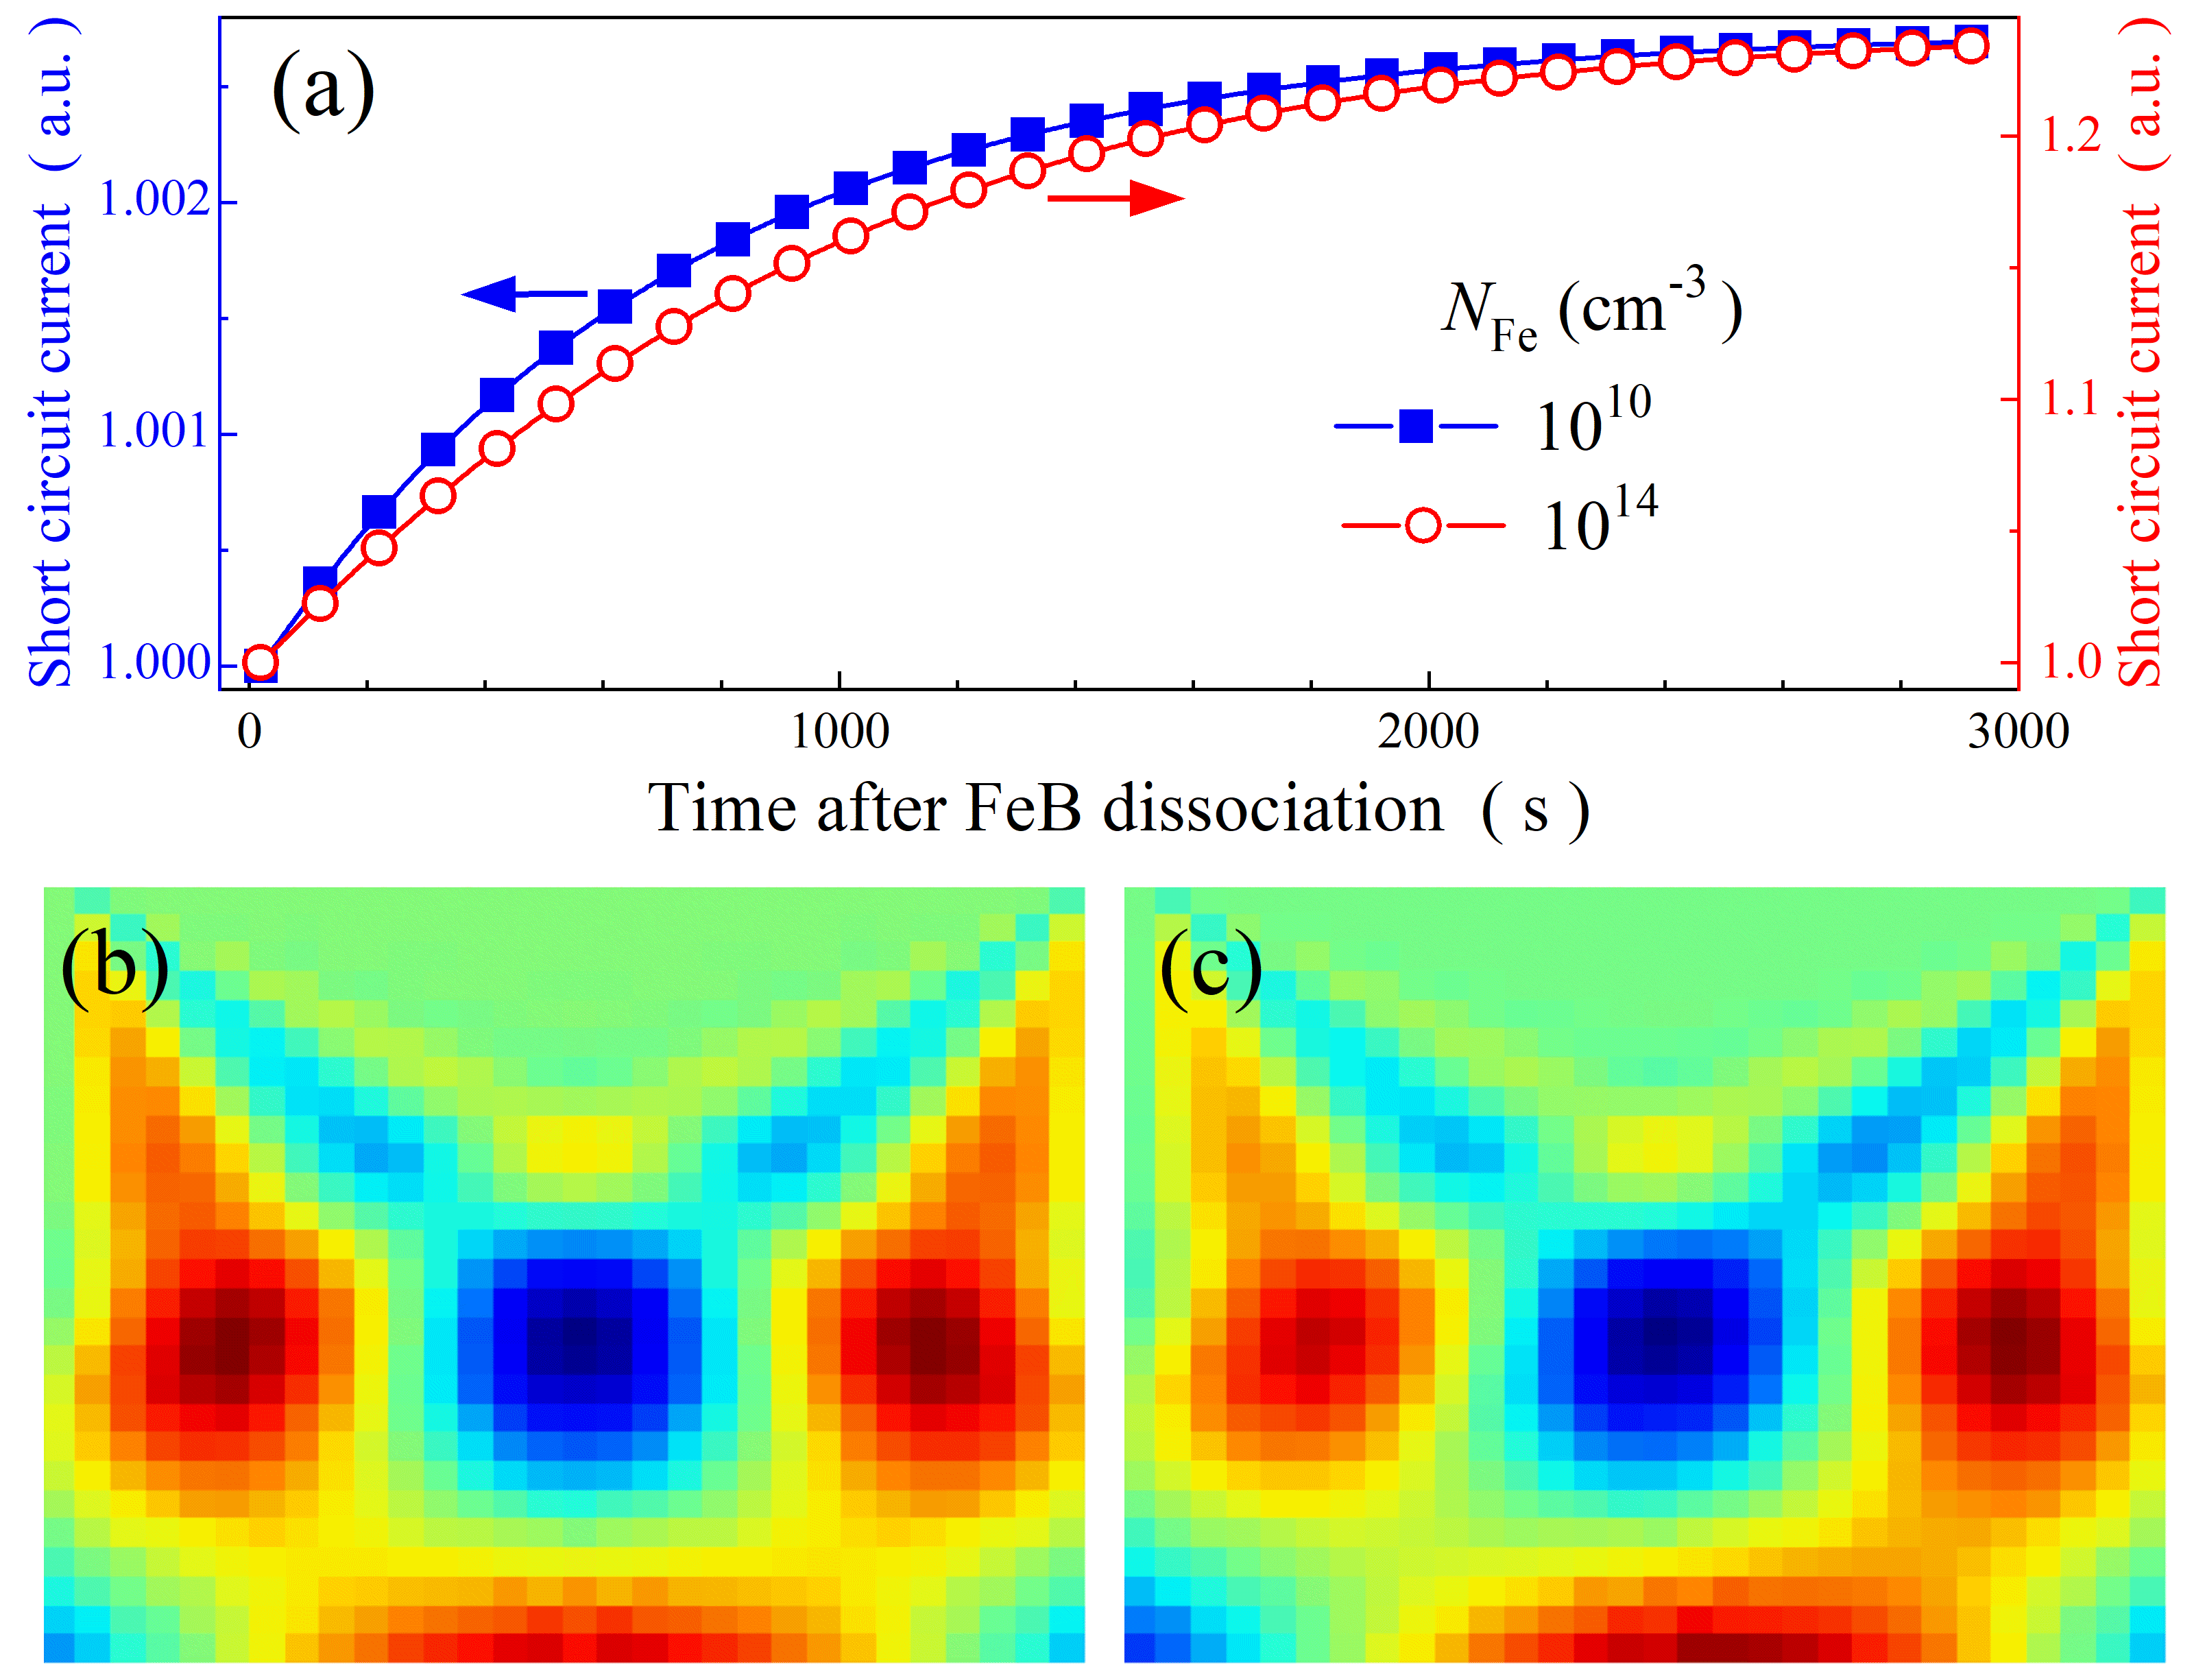
\includegraphics[width=0.5\textwidth]{Fig2}
\caption{\label{Fig2}
Simulated time dependencies of the short-circuit current (a)
and the corresponding wavelet spectrograms for iron concentrations
of $10^{10}$~cm$^{-3}$ (b) and $10^{14}$~cm$^{-3}$ (c).
The data in panel a are shown with filled squares for the concentration corresponding to panel b
and with open circles for that corresponding to panel c.
}%
\end{figure}


During the CNN Feature Processing stage, all images (both original and augmented) were processed using one of the standard CV models
to extract a feature set for each image.
The selected models and feature extraction settings are described in Subsection~\ref{subsec:CompVisMod}.
No CNN fine-tuning was performed; the models were used in their pre-trained form as downloaded.
In general, the dimensionality of the feature vectors obtained from CNN outputs substantially exceeds the number of available samples,
implying a high degree of redundancy.
Therefore, to enable comparison and mitigate this effect, Principal Component Analysis (PCA) was applied in some cases
to reduce the feature dimensionality with negligible loss of total variance.


The obtained feature sets served as inputs to regression models based on one of the standard algorithms described in Subsection~\ref{subsec:RegAlg},
which aimed to predict the iron concentration ($N_\mathtt{Fe}$) in the solar cell.
In the first case, the regression models were trained on a simulated training dataset and tested on both the simulated test dataset and experimental data.
In the second case, a portion of the experimental results was used for training, while the remaining part was reserved for testing the corresponding models.
During training, feature sets derived from the original wavelet spectrograms and their augmented versions were treated as separate samples.
During testing, the median of the predicted values obtained from the original and augmented images was used as the final prediction.
Model performance was evaluated using the metrics described in Subsection~\ref{subsec:ModEva}.


\subsection{Simulation details}\label{subsec:SimDet}

To obtain the $I_\mathtt{SC}(t)$ dependencies, $I$-$V$ curve simulations were performed for a silicon $n^+$-$p$-$p^+$ structure
under monochromatic illumination using SCAPS-1D version 3.3.11.
The SCAPS-1D software \cite{SCAPS1} is a widely used tool for modeling solar cells 
while accounting for defect states \cite{MasumMia2025, Joshi2024, Ravidas2024, Liu2024, You2023, SCAPSDefect3}.
$I_\mathtt{SC}$ values were extracted from the simulated $I$-$V$ curves using a standard procedure \cite{SCparam2017}.

During the simulations, the base thickness of the structure was set to 380~$\mu$m, 
and boron was used as the doping element with a concentration of $N_\mathrm{B} = 1.36 \times 10^{15}$ cm$^{-3}$.
The temperature was maintained at 340~K, and monochromatic illumination with a wavelength of  940~nm and an intensity of 5~W/m$^{2}$ 
was applied, corresponding to the experimental conditions (see Subsection~\ref{subsec:ExpDet}).
One of the modeling parameters was the total concentration of iron impurity atoms, $N_\mathtt{Fe}$.
It was assumed that Fe atoms were uniformly distributed throughout the base and $p^+$ layer of the solar cell 
and could exist either in interstitial positions, with a concentration $N_\mathtt{Fe_i}$, or as FeB pairs, with a concentration $N_\mathtt{FeB}$.
The time dependence of $N_\mathtt{Fe_i}$ after pair dissociation follows the well-known expression \cite{MurphyJAP2011, Wijaranakula}:
\begin{equation}
\label{eqNFet}
N_\mathrm{Fe_i}(t)=(N_\mathrm{Fe_i,0}-N_\mathrm{Fe_i,eq})\times
\exp(-t/\tau_\mathrm{ass})+N_\mathrm{Fe_i,eq}\,,
\end{equation}
where
where $N_\mathrm{Fe_i,0}$ is the concentration of interstitial iron atoms formed due to FeB pair dissosiation, 
$N_\mathtt{Fe_i,0} = N_\mathtt{Fe_i}(t=0) = N_\mathtt{Fe}$;
$N_\mathtt{Fe_i,eq}$ is the portion of interstitial iron atoms that remain unpaired in the equilibrium state 
$N_\mathtt{Fe_i,eq}=N_\mathtt{Fe_i}(t \rightarrow \infty)$,
according to \cite{MurphyJAP2011, Wijaranakula}
\begin{equation}\label{eqFeieq}
  N_\mathtt{Fe_i,eq}=\frac{N_\mathtt{Fe}}{\left[1+N_\mathtt{B}10^{-23}\exp\left(\frac{E_b}{kT}\right)\right]
  \left[1+\exp\left(\frac{E_F-E_\mathtt{Fe_i}}{kT}\right)\right]}\,,
\end{equation}
$E_b$ is the binding energy of the FeB pairs (taken as 0.582~eV \cite{Wijaranakula}),
$E_F$ is the Fermi level,
$E_\mathtt{Fe_i}$ is the position of the donor Fe$_i$ level relative to the valence band maximum
(taken as 0.394~eV \cite{FeBAssJAP2014});
$\tau_\mathrm{ass}$ is the characteristic time of the complex association,
according to \cite{FeBKin2019,FeBAssJAP2014,FeBAssSST2011}
\begin{equation}
\label{eqTass}
\tau_\mathrm{ass}=5.7\times10^5\,\frac{\mathrm{s}}{\mathrm{K}\;\mathrm{cm}^3}\times\frac{T}{N_A}\exp\left(\frac{E_m}{kT}\right)\,,
\end{equation}
$E_m$ is the energy of Fe$_\mathtt{i}^+$ migration (taken as 0.66~eV \cite{FeBAssJAP2014,FeBKin2019,FeBAssSST2011}).
In its turn, the iron–boron pair concentration $N_\mathtt{FeB}$, was estimated from
\begin{equation}\label{eqNFeB}
  N_\mathtt{FeB}(t)+N_\mathtt{Fe_i}(t)=N_\mathtt{Fe}\,.
\end{equation}
Overall, the concentrations of iron-related defects depended not only on time but
also on their spatial position within the structure, reflecting the non-uniformity of the $(E_F-E_\mathtt{Fe_i})$ difference.

A detailed description of the modeling approach, including the values of silicon and defect parameters employed, is provided elsewhere \cite{Olikh2025MSEB, Olikh2019SM}.

To create the training dataset, 25 $N_\mathtt{Fe}$ values were selected, evenly distributed on a logarithmic scale from $10^{10}$~cm$^{-3}$ to $10^{14}$~cm$^{-3}$.
Examples of the resulting dependencies are shown in \Fref{Fig2}, along with the corresponding wavelet spectrograms.
The simulated test dataset consisted of 10 dependencies calculated for 10 $N_\mathtt{Fe}$ values not included in the training dataset.



\subsection{Experiment details}\label{subsec:ExpDet}

The proposed method was validated using measurements of $n^+$-$p$-$p^+$ silicon solar cells fabricated on 
380~$\mu$m thick $p$-type boron-doped Cz wafers ($N_\mathrm{B}=1.36\times10^{15}$~cm$^{-3}$).
The $n^+$ (0.7~$\mu$m, 20–30 $\Omega$/$\Box$) and $p^+$ (0.6~$\mu$m, 10–20 $\Omega$/$\Box$)
layers were formed by phosphorus and boron diffusion, respectively.
Details of the fabrication procedure are provided elsewhere \cite{Olikh2021JAP}.

Current–voltage curves and $I_\mathtt{SC}$ kinetics were measured with a Keithley 2450 source meter. 
A 940~nm SN-HPIR940nm-1W LED (intensity 5 W/m$^{2}$) served as a monochromatic light source, 
with its output stabilized by a W1209 thermostat and a feedback-controlled power supply.
The cell temperature was regulated by a thermoelectric cooler with an STS-21 sensor and maintained constant by a PID algorithm in the control software.
FeB-pair dissociation was induced by intense (about 7000~W/m$^{2}$) halogen-lamp illumination.
The illumination intervals were selected according to a previous study \cite{OlikhPSSA}.
The kinetics of the short-circuit current were measured in the dark at 340~K for 3000~s. 
According to Eq.~\eref{eqTass}, this interval is sufficient for the complete restoration of the iron–boron pairs to their equilibrium concentration.


\Fref{Fig3}a presents an example of a measured $I_\mathtt{SC}$(t) dependence.
The signal contains some noise because, despite using a thermostat, the LED temperature fluctuated by approximately 0.4~K.
A Savitzky–Golay filter was applied for smoothing, with the window lengths and filter order selected adaptively ccording to Krishnan and Seelamantula \cite{Krishnan2013}.
Only current values corresponding to the time points used in the simulations were retained for the wavelet transformation.
The smoothed curve is shown in \Fref{Fig3}a, 
while the remaining panels of the figure display the spectrograms obtained from the raw experimental curve and the processed dependence.

\begin{figure}
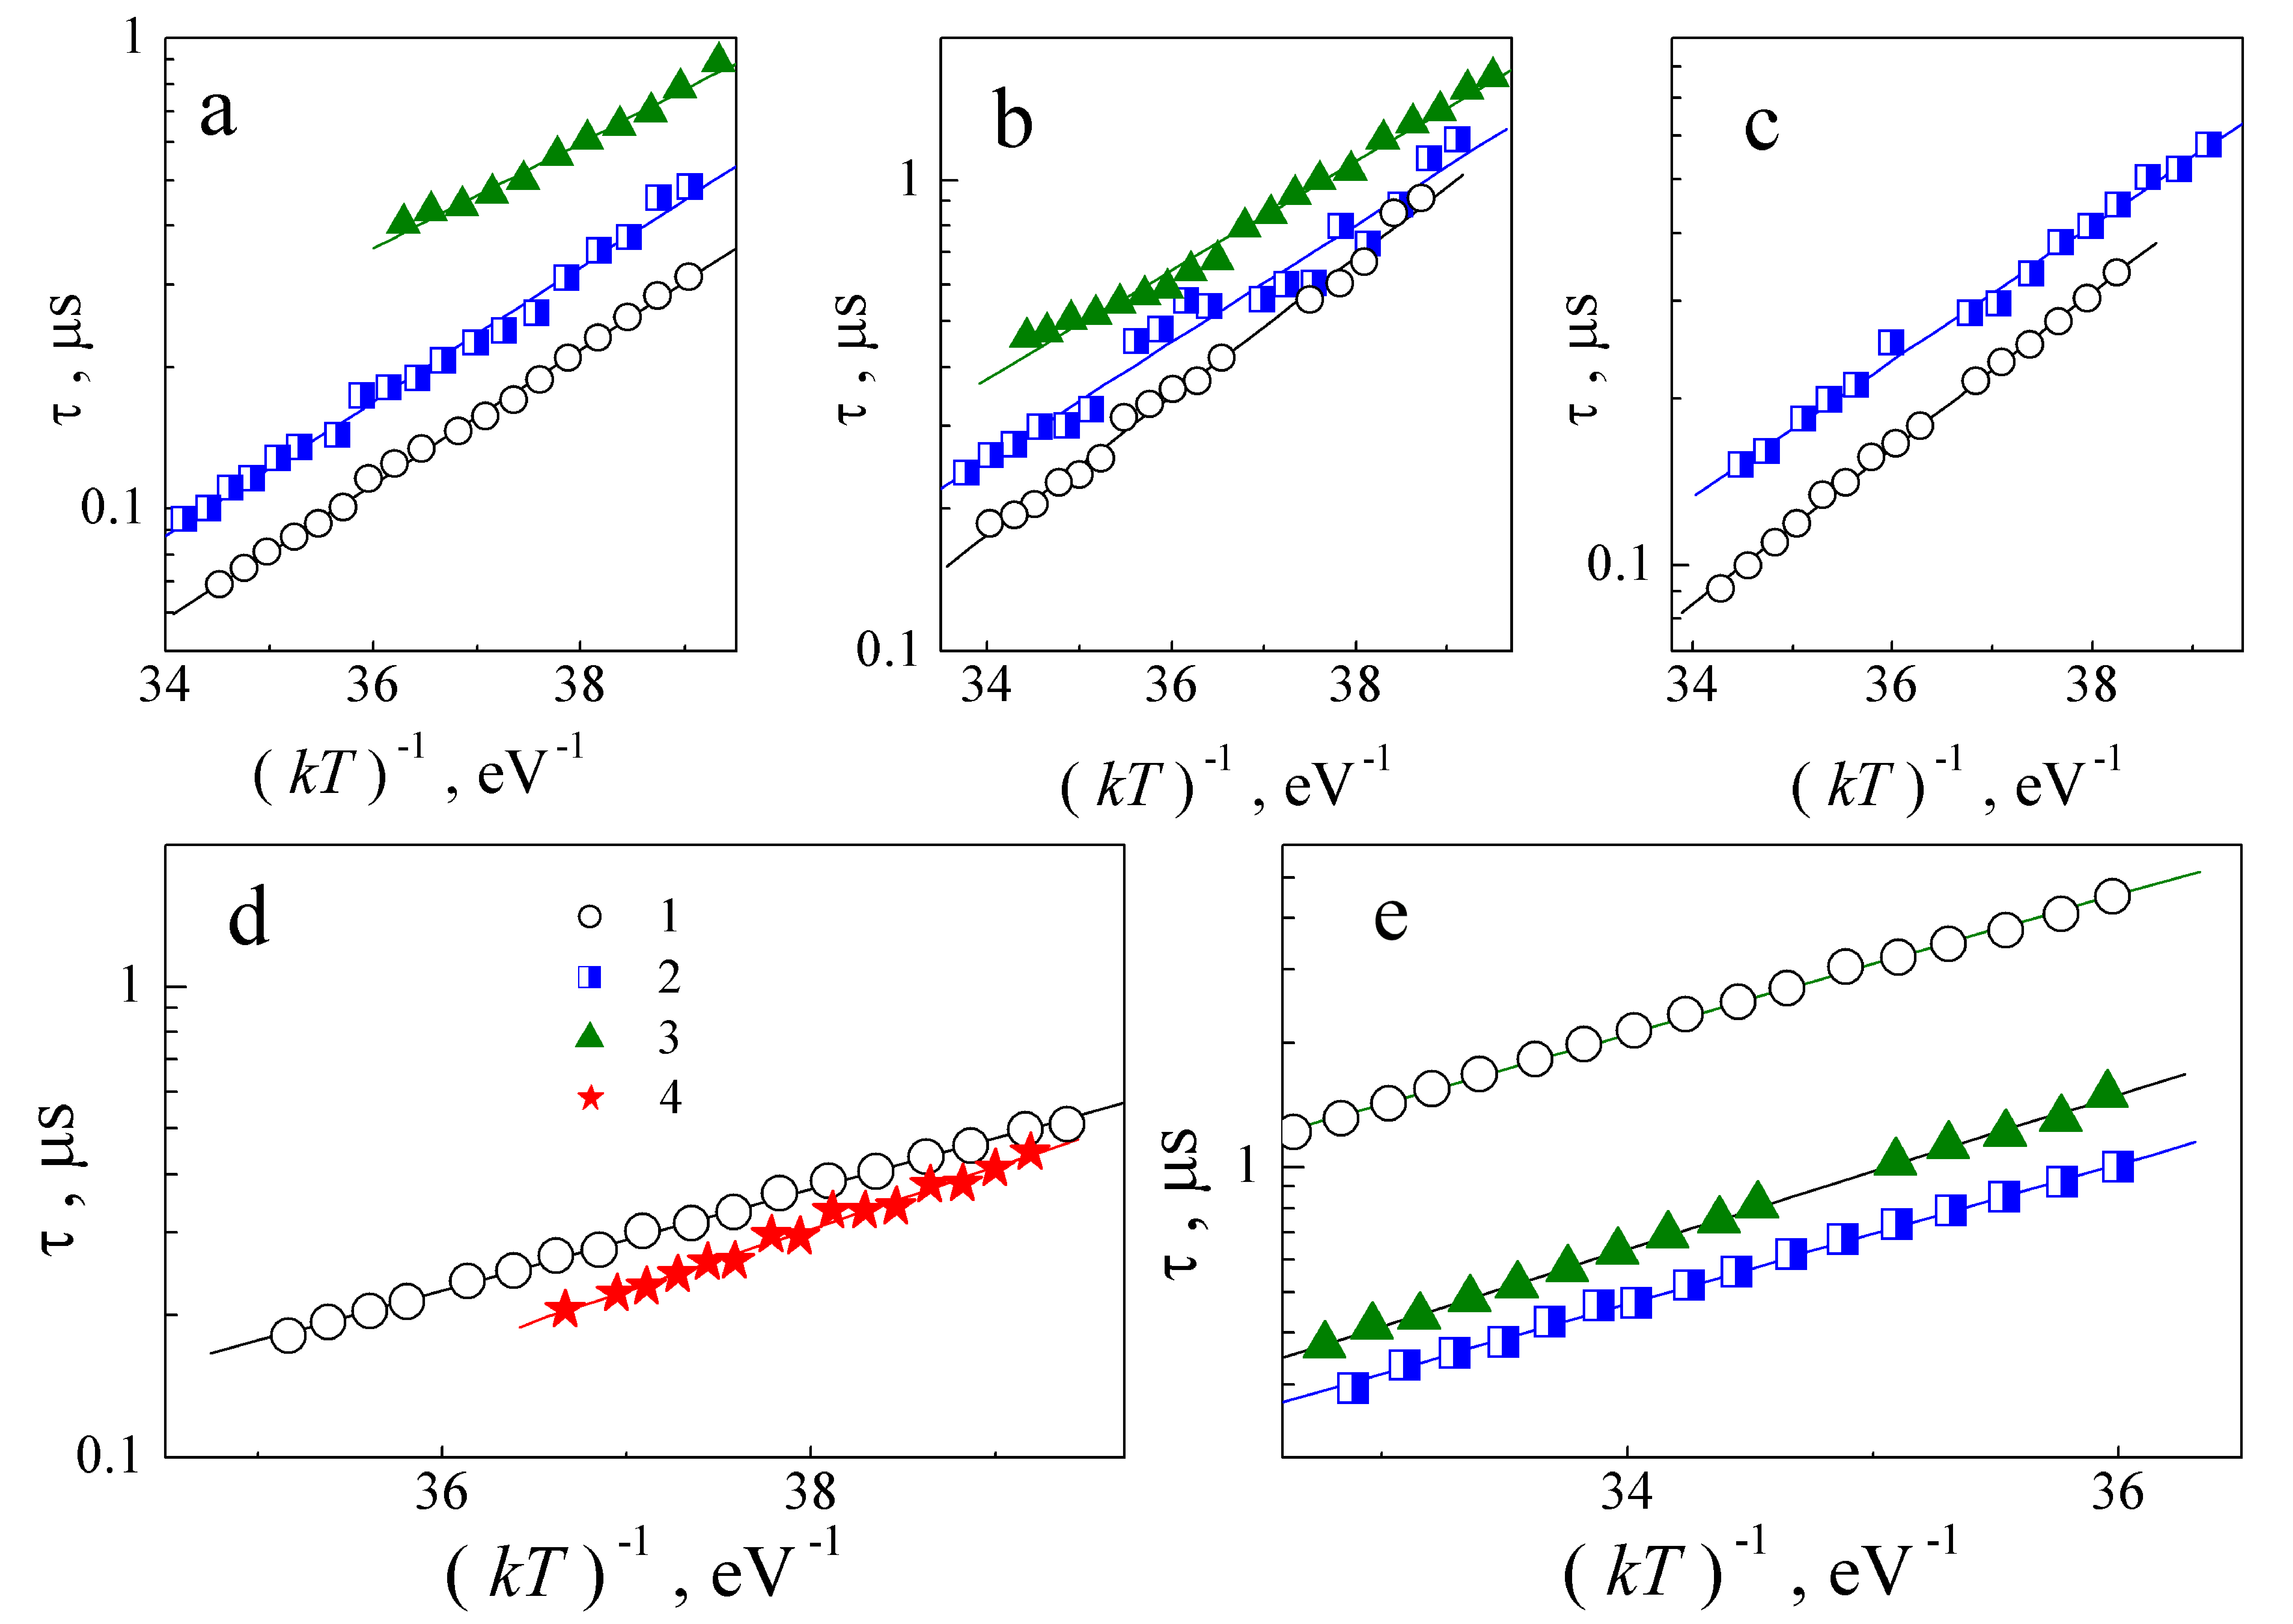
\includegraphics[width=0.5\textwidth]{Fig3}
\caption{\label{Fig3}
(a) Experimentally measured time dependence of the short-circuit current for a sample with
$N_\mathtt{Fe}=2.8\cdot10^{13}$~cm$^{-3}$ (a, open  squares) and the same dependence after applying the Savitzky–Golay filter (filled circles).
Panels (b) and (c) show the wavelet spectrograms corresponding to the curves with filled squares and open circles, respectively.
}%
\end{figure}

The iron concentration $N_\mathtt{Fe}$ was determined using a methodology described in \cite{Olikh2022:JMatSci,Olikh2021JAP}, 
which is based on fitting the kinetics of the short circuit current following FeB pairs dissociation.
A total of 28 samples with iron concentrations ranging from $10^{11}$~cm$^{-3}$ to $2\times10^{13}$~cm$^{-3}$ were examined.
To evaluate models trained on simulated data, the entire experimental dataset was used as the test set.
In cases where the models were trained using experimental data, 20 randomly selected samples were included in the training set, 
while the remaining eight samples were used for testing.



\subsection{Computer vision models}\label{subsec:CompVisMod}

To extract graphical features from the wavelet spectrograms, several computer vision models available in Keras were employed, 
namely EfficientNetB7, ResNet152V2, MobileNetV2, Xception, and NASNetLarge.
Although these models have different architectures, they all belong to the CNN class, are designed for object classification, 
and have previously been applied successfully to processing EL images of solar cells \cite{Jia2024, Otamendi2021, Chen2022, Abdelsattar2025, tella2025}.
Two feature extraction strategies were evaluated for all models: 
in the first, the class-specific probability distributions (soft labels) were passed to the subsequent stage of the pipeline, 
while in the second, the raw feature vectors directly extracted by the computer vision model were utilized.

Furthermore, the CSPDarknet53 model was employed, 
which serves as the CNN backbone for YOLOv4. 
Models of this family feature a more sophisticated CNN architecture optimized not for single-object classification 
but for multi-object detection in images. 
They are widely used in imaging-based techniques \cite{Liu2024a, Li2024a, Chen2022}. 
The employed model produces three feature maps, and for subsequent processing, either only the highest-level layer or the two deepest layers were selected.

It is well known that increasing the feature dimensionality does not necessarily enhance the total information variance. 
To mitigate the impact of redundant data, Principal Component Analysis (PCA) was applied, which constructs new, uncorrelated features (principal components). 
PCA is a widely used and effective technique in machine learning, particularly for improving performance in Electrical Testing Techniques \cite{Fadhel2019, Gao2020}. 
In this study, PCA was applied to the training datasets with an explained variance threshold of 99.9\%. 
In other words, the principal components explaining no less than 99.9\% of the total variance in the original features were selected, 
thus achieving a substantial reduction in feature dimensionality. 
This pre-processing procedure was selectively applied to a subset of the computer vision models --- 
specifically, those demonstrating good performance on the test sets without PCA --- with the aim of assessing the feasibility and effectiveness of this approach.

Given the remarkably high dimensionality of the features produced by YOLOv4, 
the feasibility of applying an alternative dimensionality reduction technique was examined. 
Specifically, global average pooling was applied to each convolutional feature map, 
replacing the spatial map with its mean value and thereby yielding a single scalar value per channel.

The configurations of the computer vision models used in this study are summarized in \tref{tabUsedMod}. 
The table also lists the notations that are subsequently used to refer to these configurations.


\begin{table*}
\centering
\caption{Summary of used pretrained CV models and feature extraction variants \label{tabUsedMod}}
\begin{indented}
\item[]
\begin{tabular}{p{2.5cm}p{4.5cm}ccc}
\br
Base model &   Model type &   Feature processing &   Output dimension &   Model Label \\ 
\mr
EfficientNetB7 & Classifier        & None & 1000 & ENB7:CL   \\ 
               & Feature extractor & None & 2560 & ENB7:FE   \\ 
               &                   & PCA  & 39   & ENB7:FE:P \\ 
MobileNetV2    & Classifier        & None & 1000 & MNV2:CL   \\ 
               & Feature extractor & None & 1280 & MNV2:FE   \\ 
               &                   & PCA  & 124  & MNV2:FE:P \\ 
NASNetLarge    & Classifier        & None & 1000 & NAS:CL    \\ 
               &                   & PCA  & 30   & NAS:CL:P  \\ 
               & Feature extractor & None & 4032 & NAS:FE    \\ 
ResNet152V2    & Classifier        & None & 1000 & R152:CL   \\
               & Feature extractor & None & 2048 & R152:FE   \\
Xception       & Classifier        & None & 1000 & XCP:CL    \\ 
               & Feature extractor & None & 2048 & XCP:FE    \\ 
YOLOv4 \newline (CSPDarknet53)&  Feature extractor  \newline (raw, top layer)& None &86528 &  YL:FE1 \\ 
&&PCA  & 137  & YL:FE1:P  \\ 
&Feature extractor  \newline (raw, top \& penultimate layers)&None &  433640 &  YL:FE2 \\         
&&PCA  & 142  & YL:FE2:P  \\
&Feature extractor \newline (pooled, top layer)&None &  512 &  YL:FP1 \\
&Feature extractor \newline (pooled, top \& penultimate layers)& None &  1024 &  YL:FP2 \\
\br
\end{tabular}
\end{indented}
\end{table*}

\subsection{Regression algorithms}\label{subsec:RegAlg}

Five ML algorithms were employed to develop regression models for predicting iron concentration: 
Random Forest (RF), Gradient Boosting (GB), eXtreme Gradient Boosting (XGB), Support Vector Regression (SVR), and Deep Neural Network (DNN). 
The models were implemented using Python libraries: Keras for DNN, Scikit-learn for RF, GB, and SVR, and XGBoost for XGB.

Each regression model was trained using features obtained from all configurations listed in \tref{tabUsedMod} and subsequently used to make predictions. 
The only exception involved the uncompressed features extracted by YOLOv4, for which the available computational resources 
(2.9 GHz AMD Ryzen 7 4800H CPU, 8 GB RAM, GeForce GTX 1650 4 GB) permitted the use of SVR only.
The target variable of all models was $\log N_\mathtt{Fe}$. 
Such logarithmic transformation is a standard approach for achieving higher prediction accuracy 
when the target quantity spans several orders of magnitude \cite{Srivastava2023, Minagawa2024}. 
Both input features and target values were normalized to have zero mean and unit standard deviation within the training set.

For each scenario, regression models were optimized to enhance predictive performance. 
Hyperparameter tuning was performed using the Optuna toolkit, 
employing the TPE sampler and the Hyperband pruner to ensure efficient selection. 
The complete list of tuned hyperparameters and their respective search ranges is provided in Tables~S1–S5 (Supplementary Material). 
Five-fold cross-validation was implemented during model tuning, with 20\% of the training data used as a validation set 
to evaluate models trained on the remaining 80\%. 
The resulting optimal hyperparameter combinations are presented in Tables~S6–S10.

Consequently, 87 distinct combinations of computer vision and regression models were investigated. 
Each combination was subsequently trained and evaluated using both simulated and experimental data. 
To identify the results for each case, a composite label was employed, derived from the last column of \tref{tabUsedMod} 
and the abbreviated name of the regression algorithm.


\subsection{Model evaluation}\label{subsec:ModEva}

%We conducted a rigorous assessment of model performance using multiple evaluation metrics to construct a robust regression model.
%For iron quantification, we used the mean squared error (MSE), mean absolute percentage error (MAPE), median absolute percentage error (MedAPE), and the coefficient of determination (R$^2$), as defined in Eqs.~\eref{eqMSE}-~\eref{eqR2}
%
%\begin{equation}\label{eqMSE}
%  MSE = \frac{1}{N}\displaystyle\sum_{i=1}^{N} (\hat{y_i}-y_i)^2,
%\end{equation}
%
%\begin{equation}\label{eqMAPE}
%  MAPE = \frac{1}{N}\displaystyle\sum_{i=1}^{N} \frac{|N_\mathrm{Fe,PRED,i}-N_\mathrm{Fe,TRUE,i}|}{N_\mathrm{Fe,TRUE,i}}\times 100 \%\,
%\end{equation}
%
%\begin{equation}\label{eqMedAPE}
%  MedAPE = median\displaystyle\sum_{i=1}^{N} \frac{|N_\mathrm{Fe,PRED,i}-N_\mathrm{Fe,TRUE,i}|}{N_\mathrm{Fe,TRUE,i}}\times 100 \%\,
%\end{equation}
%
%\begin{equation}\label{eqR2}
%  R^2 = 1-\frac{\displaystyle\sum_{i=1}^{N} (N_\mathrm{Fe,TRUE,i}-N_\mathrm{Fe,PRED,i})^2}{\displaystyle\sum_{i=1}^{N} (N_\mathrm{Fe,TRUE,i}-\overline{{N_\mathrm{Fe,TRUE,i}}})^2},
%\end{equation}
%
%where $\hat{y_i}$ represents the predicted value for the $i$-th data point, $y_i$ is the known value for the $i$-th data point, and $N$ is the number of samples in the dataset ($N$ = 25 for the simulated training set, 20 for the experimental training set, 10 for the simulated test set, and 28 and 8 for the experimental datasets used to test models trained on the simulated and experimental sets, respectively);
%$N_\mathrm{Fe,PRED,i}$ is the predicted iron concentration, $N_\mathrm{Fe,TRUE,i}$ is the known value (either the parameter used in the simulation or obtained from experimental iron determination); $N_\mathrm{Fe,TRUE}$ is the mean of the true values in the dataset.
%
%
%We selected MSE as a primary metric for assessing model accuracy and trained the models specifically to minimise it.
%However, because computing $y_i$ involves normalisation and logarithmic transformation of $N_\mathtt{Fe}$, MSE does not fully reflect the accuracy of iron-contamination estimation.
%To complement it, we used MAPE, which measures the mean relative error.
%We also considered MedAPE, which indicates the error threshold below which 50\% of the predictions fall.
%MedAPE is more robust to individual outliers, which can strongly influence the mean error in small datasets.
%Finally, we employed $R^2$ to quantify the fraction of variance in the target variable captured by the model, indicating how well the predicted values reproduce the observed data; a value of 1 corresponds to perfect agreement.

\section{Results and discussion}\label{sec:Rez}
\subsection{Simulated data}

\subsection{Experimental data}

\section{Conclusion}

\section*{References}

\bibliographystyle{iopart-num}
\bibliography{olikh}

\end{document}

